% \documentclass[twoside]{article}
\documentclass{llncs}
%\usepackage{llncsdoc}


% ------
% Fonts and typesetting settings
\usepackage[sc]{mathpazo}
\usepackage[T1]{fontenc}
\usepackage[utf8]{inputenc}
\linespread{1.05} % Palatino needs more space between lines
\usepackage{microtype}


% ------
% Page layout
\usepackage[hmarginratio=1:1,top=32mm,columnsep=20pt]{geometry}
\usepackage[font=it]{caption}
\usepackage{paralist}
\usepackage{multicol}

% ------
% Lettrines
% \usepackage{lettrine}


% ------
% Abstract
\usepackage{abstract}
	\renewcommand{\abstractnamefont}{\normalfont\bfseries}
	\renewcommand{\abstracttextfont}{\normalfont\small\itshape}


% ------
% Titling (section/subsection)
% \usepackage{titlesec}
% \renewcommand\thesection{\Roman{section}}
% \titleformat{\section}[block]{\large\scshape\centering}{\thesection.}{1em}{}


% ------
% Header/footer
% \usepackage{fancyhdr}
% 	\pagestyle{fancy}
% 	\fancyhead{}
% 	\fancyfoot{}
% 	\fancyhead[C]{SPW 2014 $\bullet$ Twenty-second International Workshop on Security Protocols}
% 	\fancyfoot[RO,LE]{\thepage}
% CFP: http://www.wikicfp.com/cfp/servlet/event.showcfp?eventid=33620&copyownerid=44118

% ------
% Clickable URLs (optional)
\usepackage{hyperref}


% ------
% BibTex for bibliography
\usepackage[square,numbers]{natbib}
%\usepackage[square,sort&compress,authoryear]{natbib}

% ------
% Math
% \usepackage{amsthm}
\usepackage{amsmath, mathtools}
\usepackage{fixltx2e}
% \usepackage{wrapfig}
\usepackage{tikz}
\usepackage{float}
\usepackage{multirow}
%\usepackage{appendices}

\usepackage{algorithm}% http://ctan.org/pkg/algorithm
\usepackage{algpseudocode}% http://ctan.org/pkg/algorithmicx
\usepackage[compatibility=false]{caption}% http://ctan.org/pkg/caption

\newtheorem{mydef}{Definition}
\newcommand{\ignore}[1]{}
% \setlength{\parskip}{0cm plus4mm minus3mm}

% ------
% Maketitle metadata
\title{\vspace{-15mm}%
	\fontsize{24pt}{10pt}\selectfont
	\textbf{Traversing symmetric NAT with predictable port allocation function}
	}	
\author{%
	\large
	\textsc{Du\v{s}an Klinec} \\[2mm]%\thanks{Template by \href{http://www.howtotex.com}{howtoTeX.com}} \\[2mm]
	\normalsize	Faculty of Informatics \\
	\normalsize	Masaryk University, Brno \\
	\normalsize	\href{mailto:xklinec@fi.muni.cz}{xklinec@fi.muni.cz}
	\and
	\textsc{Vashek Matyáš} \\[2mm]%\thanks{Template by \href{http://www.howtotex.com}{howtoTeX.com}} \\[2mm]
	\normalsize	Faculty of Informatics \\
	\normalsize	Masaryk University, Brno \\
	\normalsize	\href{mailto:matyas@fi.muni.cz}{matyas@fi.muni.cz}
	\vspace{-5mm}
	}
\date{}



%%%%%%%%%%%%%%%%%%%%%%%%
\begin{document}

\maketitle
% \thispagestyle{fancy}

\begin{abstract}
\noindent Network Address Translators cause troubles for VoIP and other P2P services since central servers are needed for communication.
A presence of such potentially malicious hosts in a communication path is not desired, mainly due to increased cost, poor link quality 
and security consequences.
Several solution exist for traversing NAT but symmetric case is still problematic. We propose algorithms using single source port for 
symmetric NAT traversal, each with different properties and applicability. 
Paper gives a theoretic point of view on the NAT traversal problem by stating problem formally and modeling a network connected to 
NAT as a random process, in order to evaluate algorithms in a different settings.
% 
% ToDo; Will be written as the last part of the paper... Lorem ipsum dolor sit amet, consectetur adipiscing elit. Curabitur magna lorem, tempor sed facilisis vel, porta et turpis. Sed et felis a massa dictum posuere. Aliquam hendrerit rhoncus ipsum sit amet placerat. Duis fringilla est eu arcu mollis faucibus non sit amet eros. Vestibulum risus nibh, dapibus vitae laoreet eget, fringilla quis nisl. Proin consequat nibh sit amet mauris suscipit tincidunt. Sed rutrum, purus nec aliquam faucibus, quam libero venenatis nisi, ut tempor mi sapien vel diam. Pellentesque sagittis elit non risus malesuada accumsan. Morbi consequat urna.
\end{abstract}
	

% \begin{multicols}{2}
% \lettrine[nindent=0em,lines=3]{L}orem ipsum dolor sit amet. 

\section{Introduction}
Network Address Translators (abbreviated as NAT) has been increasing in popularity in recent years 
mainly as a mean of slowing down IPv4 address space depletion. On one hand NAT offers
the ability to share a public, globally routable IP address among many internal network hosts. On 
the other hand it breaks basic end-to-end principle of the Internet and thus favors server-client 
communication model for clients connected behind NAT.

In many applications is a peer-to-peer (P2P) connection of crucial importance and the quality of a service depends on 
its parameters heavily. Main motivation for this work is Voice-over-IP (VoIP) where direct connection 
between communicating parties is necessary. If P2P connection is not possible to be established, relay 
servers has to be used (TURN~\citep{rfc5766} protocol is used). The presence 
of another node in the communication path can have negative effects on a communication channel quality 
(increased latency, jitter, lower bandwidth), relay server is a potential point of failure, 
has to scale with increasing demands of the network, etc...
Thus relay servers require non-negligible resources what makes them expensive for VoIP providers and
establishing a direct connection between parties is of high importance.

From an attacker perspective, relay servers are interesting point where to attack thus from security
standpoint they could be seen as potential enemies trying to sniff and log all 
communication. NAT (especially symmetric one, used as a carrier-grade border firewall in large networks)
forces communicating parties to use such central servers
for communication making monitoring easier for an attacker. Traversal algorithms has to collaborate 
with central servers in such a way they create a direct link, not using servers any further. 
% 
% some way. They use it to create a direct link, not using servers any further. 

In this paper we are focused on a symmetric NAT with a predictable port allocation function. We propose 
new algorithms for establishing direct connection between hosts behind such NATs that are effective and 
has low system requirements.

\section{Existing techniques}
Many different solutions for traversing non-symmetric NATs exist e.g., NAT traversal in Internet Key Exchange~\citep{rfc3947} or 
Interactive Connectivity Establishment~(ICE)~\citep{rfc5245}. %Terredo\ignore{tunneling}~\citep{rfc4380}.

Some devices with NAT functionality provide special interface enabling traversal, for example NAT Port Mapping Protocol~\citep{rfc6886}. But in general 
it is not widely deployed and it cannot be relied upon in a general case. 

Most of the applications use ICE\ignore{~\citep{rfc5245}} nowadays, what is a very powerful toolbox for traversing 
various types of NAT, however does not work with symmetric NATs. ICE mainly uses STUN~\citep{rfc5389} and TURN\ignore{~\citep{rfc5766}} for its operation.

% \section{Related work}
Some interesting algorithms for traversing symmetric NAT were proposed by Y.~Takeda in \citep{takeda}, but the case both clients are behind symmetric NAT
with port sensitive allocation function is not covered. It mentions that sending more packets does not increase a probability of establishing a new connection.
Our motivation is to show that it is actually possible.

RFC~5128 \citep{rfc5128} maps current state of the art in NAT traversal, but does not cover our case. 
The research by Wei~\emph{et.~al.} in \citep{wei}., is devoted to symmetric NAT traversal but their algorithm is using another technique compared
to our approach. The downside of their algorithm is it requires Time To Live~(TTL) modification of the IP~packet. This is usually considered
as a privileged operation in the operating system and super-user privileges are required for this modification. 

Wang~\emph{et.~al.} \citep{Wang:2006:RSN:1156422.1156550} propose a NAT traversal algorithm for setting we are using based on
a changing of a source port, while in our approach we want to explore possibilities with constant source port.

In our work we study the situation where two parties, A,B tries to establish a direct connection, both of them are behind 
a symmetric NAT (possibly cascade of such NATs) with port sensitive, predictable allocation function. Another scenarios with
predictable allocation function are quite easy to solve and covered in previous research. 

\section{Network Address Translation}
The notation used for the rest of the paper follows.

% \paragraph{Notation.}
% Symmetric NAT could be defined as follows.

\begin{mydef}
\begin{align*}
\mathbb{SC} = \mathbb{IP} \times \mathbb{PORT}
\end{align*} is a Socket. $\mathbb{IP}$ is set of all possible IP addresses and $\mathbb{PORT}$ 
is set of all possible ports, basically $\mathbb{PORT} = \{1,2,\dots,65535\}$.
\begin{align*}
\mathbb{SP} = \mathbb{IP} \times \mathbb{PORT} \times \mathbb{IP} \times \mathbb{PORT}
\end{align*} is a Socket Pair.
\end{mydef}
% 
% \begin{mydef}
% \begin{align*}
% \mathbb{AT} \subseteq \mathbb{SP} \times \mathbb{PORT}
% \end{align*} is an allocation table of the NAT. Second component is external port allocated for particular socket pair.
% \end{mydef}
% Allocation table is a set of all socket pairs and corresponding allocated external port.

\paragraph{NAT and communication.}
NAT connects two networks, denoted as an internal and an external, connected to an internal and an external NAT interface respectively.
Hosts has addresses $\text{IP\textsubscript{in}} \in \mathbb{IP}_{in} \subseteq \mathbb{IP}$ 
and $\text{IP\textsubscript{ex}} \in \mathbb{IP}_{ex} \subseteq \mathbb{IP}$ in the internal and the external network
respectively, $\mathbb{IP}_{in} \cap \mathbb{IP}_{ex} = \emptyset$.
If it is not said otherwise the external NAT address\footnote{We assume NAT has only one external address for simplicity.} is denoted as 
$\text{IP\textsubscript{nat}} \in \mathbb{IP}_{ex}$.

Packet received on the external interface has socket pair {(IP\textsubscript{ex},PORT\textsubscript{ex},IP\textsubscript{nat},PORT\textsubscript{nat})}.

Packet received on the internal interface has socket pair {(IP\textsubscript{in},PORT\textsubscript{in},IP\textsubscript{ex},PORT\textsubscript{ex})}.

% \paragraph{Filtering rule.} Let assume packet with socket pair {(IP\textsubscript{out},PORT\textsubscript{out},IP\textsubscript{ex},PORT\textsubscript{ex})} 
% received on NAT external interface (we'll use this notation in further text). Packet is allowed to pass to internal network iff 
% \begin{align*}
% &  \exists \; \text{IP\textsubscript{in}} \in \mathbb{IP}, \; \text{PORT\textsubscript{in}} \in \mathbb{PORT}:\\
% & ((\text{IP\textsubscript{in}}, \text{PORT\textsubscript{in}}, \text{IP\textsubscript{out}}, \text{PORT\textsubscript{out}}), \text{PORT\textsubscript{ex}} ) \in \mathbb{AT}
% \end{align*}
% 
% If packet is allowed to pass, it is then forwarded to host {(IP\textsubscript{in}, PORT\textsubscript{in})}. A new record 
% to the allocation table is added when internal host sends packet to the external host. 
% 
% \paragraph{Allocation rule.} ToDo

\subsection{NAT classes}\label{sec:nat}
NAT is classified w.r.t. \emph{filtering rule} and \emph{allocation rule} which says what happens after receiving
packet from an external and an internal network respectively.

Common NAT categorization is according to~\citep{rfc3489}: a) Full Cone
b) IP Restricted Cone, c) Port Restricted Cone, d) Symmetric.

% MOVED TO APPENDIX
% \paragraph{Full cone NAT.} ~\\
% Allocation table $\mathbb{AT} \subseteq \{ \mathbb{IP}_{in} \times \mathbb{PORT} \} \times \mathbb{PORT}$ holds associations between internal 
% hosts socket and mapped external NAT port. 
% % Rule is created once the connection from the internal host is initiated to an arbitrary external address.
% Filtering rule is:
% \begin{align*}
% & PASS((\text{IP\textsubscript{ex}}, \text{PORT\textsubscript{ex}}, \text{IP\textsubscript{nat}}, \text{PORT\textsubscript{nat}} )) \Leftrightarrow \\
% &  \exists \; \text{IP\textsubscript{in}} \in \mathbb{IP}_{in}, \; \text{PORT\textsubscript{in}} \in \mathbb{PORT}:\\
% & ((\text{IP\textsubscript{in}}, \text{PORT\textsubscript{in}}), \text{PORT\textsubscript{nat}} ) \in \mathbb{AT}
% \end{align*}
%  
% \paragraph{Address restricted cone NAT.} ~\\
% Allocation table $\mathbb{AT} \subseteq \{\mathbb{IP}_{in} \times \mathbb{PORT} \times \mathbb{IP}_{ex}\} \times \mathbb{PORT}$ 
% holds associations between internal hosts socket, external host IP address and mapped external NAT port. 
% % Rule is created once the connection from the internal host is initiated to an arbitrary external address.
% Filtering rule is:
% \begin{align*}
% & PASS((\text{IP\textsubscript{ex}}, \text{PORT\textsubscript{ex}}, \text{IP\textsubscript{nat}}, \text{PORT\textsubscript{nat}} )) \Leftrightarrow \\
% &  \exists \; \text{IP\textsubscript{in}} \in \mathbb{IP}, \; \text{PORT\textsubscript{in}} \in \mathbb{PORT}:\\
% & ((\text{IP\textsubscript{in}}, \text{PORT\textsubscript{in}}, \text{IP\textsubscript{ex}}), \text{PORT\textsubscript{nat}} ) \in \mathbb{AT}
% \end{align*}

\paragraph{Port restricted cone NAT.} ~\\
Allocation table $\mathbb{AT} \subseteq \{\mathbb{IP}_{in} \times \mathbb{PORT} \times \mathbb{IP}_{ex} \times \mathbb{PORT}\} \times \mathbb{PORT}$ 
holds associations between internal hosts socket, external host socket and mapped external NAT port. 
% Rule is created once the connection from the internal host is initiated to an arbitrary external address.
Filtering rule is:
\begin{align*}
& PASS((\text{IP\textsubscript{ex}}, \text{PORT\textsubscript{ex}}, \text{IP\textsubscript{nat}}, \text{PORT\textsubscript{nat}} )) \Leftrightarrow \\
&  \exists \; \text{IP\textsubscript{in}} \in \mathbb{IP}, \; \text{PORT\textsubscript{in}} \in \mathbb{PORT}:\\
& ((\text{IP\textsubscript{in}}, \text{PORT\textsubscript{in}}, \text{IP\textsubscript{ex}}, \text{PORT\textsubscript{ex}}), \text{PORT\textsubscript{nat}} ) \in \mathbb{AT}
\end{align*}

\paragraph{Symmetric NAT.} ~\\
Allocation table $\mathbb{AT}$ and filtering rule is the same as in Port restricted Cone NAT. The difference lies in the way 
the new entries in the allocation table are created. For Cone NAT holds that multiple entries in the allocation table 
can have the same external port assigned, while Symmetric NAT creates new allocation entries under certain circumstances.

\emph{Allocation function (AF)} defines port allocation rules for new connections (not in $\mathbb{AT}$). Assume $\mathbb{AT}=\emptyset$, for simplicity. 
AF can be either \emph{predictable} or \emph{random}. In our setting predictable AF is assumed, e.g., \emph{incremental}. 
If previously allocated port was $\text{PORT\textsubscript{nat}}$
the next port will be $\text{PORT\textsubscript{nat}}+\Delta$, where $\Delta=1$ usually.
If the chosen port is already taken, AF iterates until the free one is found.

AF can have different \emph{sensitivity} determining the cases where new allocation is created or the previous one is used instead.

\emph{Address sensitive allocation function} creates new allocation if a destination address differs from the existing allocation 
from the same source:
\begin{align*}
& \exists s=(a_1,a_2,a_3,a_4) \in \mathbb{SP}, p \in \mathbb{PORT}: \\
& (s, p) \in \mathbb{AT} \Rightarrow ((\forall s^{\prime}=(a_1^{\prime},a_2^{\prime},a_3^{\prime},a_4^{\prime}) \in \mathbb{SP}, \\
& a_1 \neq a_1^{\prime}, a_2 \neq a_2^{\prime}, a_3 \neq a_3^{\prime}, \forall p^{\prime} \in \mathbb{PORT}: \\
& ((s^{\prime}, p^{\prime}) \in \mathbb{AT})) \Rightarrow p \neq p^{\prime})
\end{align*}

\emph{Port sensitive allocation function} creates new allocation if a destination address and a port differs from the existing
allocations from the same source:
\begin{align*}
& \exists s \in \mathbb{SP}, p \in \mathbb{PORT}: (s, p) \in \mathbb{AT} \Rightarrow \\
& \Rightarrow ((\forall s^{\prime} \in \mathbb{SP}, s^{\prime} \neq s , \forall p^{\prime} \in \mathbb{PORT}: \\
& ((s^{\prime}, p^{\prime}) \in \mathbb{AT})) \Rightarrow p \neq p^{\prime})
\end{align*}
% 
%     PASS((\text{IP\textsubscript{out}}, \text{PORT\textsubscript{out}}, \text{IP\textsubscript{ex}}, \text{PORT\textsubscript{ex}} )) \Leftrightarrow \\
% &  \exists \; \text{IP\textsubscript{in}} \in \mathbb{IP}, \; \text{PORT\textsubscript{in}} \in \mathbb{PORT}:\\
% & ((\text{IP\textsubscript{in}}, \text{PORT\textsubscript{in}}, \text{IP\textsubscript{out}}, \text{PORT\textsubscript{out}}), \text{PORT\textsubscript{ex}} ) \in \mathbb{AT}
% \end{align*}

% \section{Related work II}
% \begin{compactitem}
% \item chineese\citep{Wang:2006:RSN:1156422.1156550}
% \item uPNP
% \item PCP~\citep{rfc6887}
% \end{compactitem}

\section{UDP hole punching with STUN}
All algorithms in our paper make use of the same principle, \emph{UDP hole punching}. 
Internet hosts cannot send packet to the internal host directly. 
Communication has to be initiated from the inside\footnote{Not taking
pre-set port forwarding, DMZ, uPnP, etc... into consideration. }, what is problematic if two nodes behind 
NAT wants to communicate.

Assume two parties, A and B with addresses IP\textsuperscript{A} and IP\textsuperscript{B} respectively,
A and B are behind public NAT with addresses $\text{IP}^{\text{A}}_{\text{nat}}$ and $\text{IP}^{\text{B}}_{\text{nat}}$
respectively. By default an internal host does not known its external address and NAT type thus technique like 
STUN\footnote{Core idea: publicly available service running on 2 IP addresses and 2 ports 
answering questions like: what is my IP address and port? Change IP address of response if I'll get it, etc...} 
is used to learn it. In case of incremental NAT it is also needed to determine $\Delta$ and the next port
that is likely to be allocated for a new connection $\text{PORT}^{\text{A}}_{\text{nat}}$ for A and $\text{PORT}^{\text{B}}_{\text{nat}}$
for B. The period between determining this information, sending to the other party and starting the algorithm is
denoted as an \emph{initialization phase} or a \emph{silent period}\ignore{\footnote{Since the algorithm itself does nothing.}} of the NAT traversal algorithm. 

UDP hole punching works as follows:\\
\begin{compactitem}
 \item [1.] $A: \; IP^A_{in}:PORT^A_{in} \longrightarrow IP^B_{nat}:PORT^B_{nat}$ \\
Locally a~new mapping is created ($PORT^A_{nat}$), packet is dropped on B's~NAT.
 \item [2.] $B: \; IP^A_{nat}:PORT^A_{nat} \longleftarrow  IP^B_{in}:PORT^B_{in}$ \\
Locally a~new mapping is created ($PORT^B_{nat}$), packet reaches A using allocation created in step~1.
 \item [3.] $A: \; IP^A_{in}:PORT^A_{in} \longrightarrow IP^B_{nat}:PORT^B_{nat}$ \\
Packet reaches B using allocation created in in step~2.
\end{compactitem}

% By default a packet 
% coming from the internet (\textit{IP\textsubscript{A},Port\textsubscript{A}}) to the internal 
% network is dropped on the NAT unless there is a valid mapping in NAT allocation table.

\section{Theoretical network model}
In order to evaluate algorithms in multiple environments with different parameters (workload, number of clients, etc.)
we decided to model network behavior with stochastic process. In particular we choose a Poisson process, $\{N(t), t\geq0\}$ 
that is used in queueing theory to model arrivals of requests to the server queue~\citep{Nelson:1995:PSP:207382}. 

The core idea of NAT traversal is to predict the next allocated external port by NAT, thus from this perspective 
it is important to model how NAT's internal state changes over time, i.e., how many external ports 
were allocated in a given time interval. Thus the workload is important parameter for predicting an allocated port.

We model internal network connected to NAT w.r.t. newly created connections (new port allocation) as a 
time homogeneous Poisson process $Po(\lambda)$. By setting $\lambda$ we can model 
different workload of the network and evaluate algorithms with respect to the various parameters e.g., 
probability of an establishing connection. 

% Random variable $X_t \sim Po(\lambda t)$ says how many
% port allocations were made in time interval $[0,t]$

\begin{mydef}
$N(t)$ is a random variable of a number of a new port allocations made in time 
interval~$[0,t]$ where $N(t) \sim Po(\lambda t)$. \\ 
                                                      
\begin{center}                                                     
Then $P[N(t)=n] = \frac{(\lambda t)^n}{n!} e^{-\lambda t}$
\end{center}
\end{mydef}

Moreover we assume incremental NAT with $\Delta=1$ on both sides. If we sample the NAT 
state\footnote{STUN request to determine current port number, it creates a new NAT allocation record.}
each $T=10$~milliseconds the NAT state can be modeled as a random process $\{C_i | C_i \in \mathbb{N}, C_i \geq i, i\geq0\}$ where:
\[
C_i = \begin{dcases*}
         0 & if $i=0$ \\
         C_{i-1} + 1 + X_i, \; X_i \sim Po(\lambda T) & otherwise 
        \end{dcases*}
\]
Rewritten as $C_i = i + \sum_{j=1}^{i}X_j$. Expected value $E[C_i] = i + E[\sum_{j=1}^{i}X_i] = i (1+\lambda T)$.

\paragraph{Port pool exhaustion.} NAT timeout\footnote{Allocation is deleted if no packet is detected in this time interval.} is assumed to be 3~minutes, 
what is common value in practice. This constrains $\lambda$ to the interval $[0, 0.36]$, intuitively from $0$ to $360$ new connections in $1$~s on average. 
If it is higher the NAT is rendered as unusable since the port pool is exhausted\footnote{$P[X > 65535] = 0.0019, X \sim Po(180000 \cdot 0.36)$.} quickly.

\section{Generic algorithm structure}
Algorithms we propose have a common structure. In order to maximize probability of an establishing
a connection (i.e., success rate) it proceeds in discrete \emph{steps}. In each step it 
tries to open a new hole on the local NAT and/or to predict corresponding port allocated on the destination
NAT.

\begin{mydef}
Symmetric NAT traversal algorithm is a mapping 
$\mathcal{A}: \mathcal{U} \times \mathcal{S} \times \mathcal{M} \rightarrow \mathcal{P}_{src} \times \mathcal{P}_{dst}$, 
where \\
\begin{compactitem}
\item $\mathcal{U}=\{0,1\}$ is set of communicating parties.
\item $\mathcal{S} = \{0, 1, \dots, n-1\}, \; n \in \mathbb{N}$ is a step of the algorithm.
\item $\mathcal{M}$ is set of vectors of parameters of the environment (i.e., network model 
parameters and additional information obtained in initial phase). 
In our setting $\mathcal{M} = \{ (\lambda, t_s) | \lambda~>~0, t\geq~0 \}$. Value $t_s$ is length of the silent period. %For simplicity $\mathcal{M} = \{ \lambda | \lambda > 0 \}$.
\item $\mathcal{P}_{src} \subseteq \mathbb{N}$ and $\mathcal{P}_{dst} \subseteq \mathbb{N}$
are sets of source and destination ports respectively.
\end{compactitem}
\end{mydef}
If the third parameter is not important for the algorithm it can be ignored in the notation. 

Prior algorithm run it is needed to 
determine NAT state (for UDP hole punching), this is assumed to be done by some technique like STUN. For simplicity we assume the port numbers
starts from $0$. The length of the silent period is also known to the algorithm prior execution in order to estimate the current state of 
the NAT, e.g., difference between the last measurement and just before algorithm execution.

\paragraph{Intuition.} 
Line $A(0,1) = (2,3)$ means party $0$ in step $1$ sent packet from source port $2$ to destination port $3$
of the party $1$.

\paragraph{Time.} 
%The algorithm proceeds in discrete time steps. 
Algorithm starts in time $t_0 = 0$~ms and each step $i \in \mathcal{S}$
happens in time $t_i = iT$ for some $T$. If it is not mentioned otherwise, $T = 10$~ms.

%\paragraph{Party change.} 
%We define unary operation on communicating parties. 
%\[
%a \in \mathcal{U},  \neg a = \begin{dcases*}
%         0 & when $a=1$\\
%         1 & when $a=0$
%        \end{dcases*}
%\]

\paragraph{Algorithm log \& successful run.} IP addresses of the hosts and NAT are known and fixed prior algorithm run thus omitted
from the notation for simplicity. For the following text is assumed maximum number of steps of the algorithm $s_{max}=1000$.

\begin{mydef}
\label{def:log}
Algorithm log $\mathcal{L}^A_{\mathcal{A}}$ is a set of tuples $(p_1, p_2, p_3) \in \mathcal{L}^A_{\mathcal{A}}$ produced
by the NAT traversal algorithm $\mathcal{A}$ execution on the host $A$, where: \\
%$\mathcal{A}(0, s, (\lambda, t_s)) = (p_1, p_2)$ 
%are generated by $\mathcal{A}$ for some parameters $\lambda, t_s$ in some step $s$. The $p_3$ is 
%an allocated port by $NAT^A$ for request $(p_1, p_2)$ in a given step. Algorithm log for host $B$ is defined analogically. 
%Furthermore from our setting the 
%following formula holds:\footnote{From definition of a port sensitive symmetric NAT.} %$\mathcal{L^{A}} \subseteq PORT_{in}^{A} \times PORT_{nat}^{B} \times PORT_{nat}^{A}$, 

\begin{compactitem}
 \item $(p_1, p_2) = \mathcal{A}(0, s, (\lambda, t_s)) $ are generated by the algorithm $\mathcal{A}$ for some 
       parameters $(\lambda, t_s)$ in some step $s$ of the algorithm $\mathcal{A}$.
 \item $p_3$ is an allocated port by $NAT^A$ for request $(p_1, p_2)$ in a given step $s$. In our network model
       $p_3=C_s=C_{s-1} + 1 + X, X~\sim~Po(\lambda T)$.
 \item Algorithm log for host $B$ is defined analogically.
 \item Furthermore from our setting the following formula holds:\footnote{From definition of a port sensitive symmetric NAT.}
\end{compactitem} %
%
% \begin{compactitem}
% \item $p_1$ is a source port.
% \item $p_2$ is a destination port.
% \item $p_3$ is an allocated port by local NAT for this request.
% \item following formula holds\footnote{from definition of a port sensitive symmetric NAT}
% \end{compactitem}
%
\begin{align*}
& (p_1, p_2, p_3) \in \mathcal{L}^A_{\mathcal{A}}: \forall (p_1^{\prime}, p_2^{\prime}, p_3^{\prime}) \in \mathcal{L}^{A}_{\mathcal{A}} :\\
& p_3 = p_3^{\prime} \Leftrightarrow \left( p_1=p^{\prime}_1 \wedge p_2=p^{\prime}_2 \right)
\end{align*}
\end{mydef}

\begin{mydef}
\label{def:match}
Algorithm $\mathcal{A}$ run is successful, i.e., established a direct connection between $A,B$ if\footnote{Derived from UDP hole punching.}:
\begin{align*}
& MATCH(\mathcal{L}^{A}_{\mathcal{A}}, \mathcal{L}^{B}_{\mathcal{A}}) \Leftrightarrow \exists(p_1, p_2, p_3) \in \mathcal{L}^{A}_{\mathcal{A}}: \\
& \exists(p_1^{\prime}, p_2^{\prime}, p_3^{\prime}) \in \mathcal{L}^{B}_{\mathcal{A}}: p_2 = p_3^{\prime} \wedge p_2^{\prime} = p_3
%
%  \in \mathcal{L}^A_{\mathcal{A}}: \forall (p_1^{\prime}, p_2^{\prime}, p_3^{\prime}) \in \mathcal{L}^{A}_{\mathcal{A}} :\\
%& p_3 = p_3^{\prime} \left( \Leftrightarrow p_1=p^{\prime}_1 \wedge p_2=p^{\prime}_2 \right)
\end{align*}
\end{mydef}
The task is to find an algorithm $\mathcal{A}$ such that the probability the $MATCH(\mathcal{L}^{A}_{\mathcal{A}}, \mathcal{L}^{B}_{\mathcal{A}})$
holds is maximized for minimal number of steps needed.

\subsection{Algorithm I -- baby-step, giant-step}
We propose the algorithm with high success rate for small network loads, i.e.,
$\lambda \leq 0.03, T=10$~ms. When error becomes larger,
algorithm step is not fast enough to compensate errors and thus fails for larger $\lambda$.

\begin{mydef}
Baby-step giant-step algorithm
\[
u \in \mathcal{U}, s \in \mathcal{S}: 
\mathcal{A}(u, s) = \begin{dcases*}
         (0, s)  & \text{if} $u=0$\\
         (0, 2s) & \text{if} $u=1$
        \end{dcases*}
\]
\end{mydef}

Intuitively the source port is kept constant, one side of the protocol scans ports sequentially, another
side of the protocol scans ports with step 2.

\subsection{Algorithm II -- fixed destination port}
Algorithm with fixed destination port described in by \citep{Wang:2006:RSN:1156422.1156550}
changes the source port in order to create new holes in NAT in each step.

\begin{mydef}
Fixed destination port algorithm
\[
u \in \mathcal{U}, s \in \mathcal{S}: \;
\mathcal{A}(u, s) = (s, \Delta_u)
\] for some constants $\Delta_0, \Delta_1$ based on the current network workload determined in initial phase
of the protocol.
\end{mydef}

\subsection{Algorithm III -- expected port value}
Some more effective algorithms can be designed if the random process the network follows is known (and their
parameters).

\begin{mydef}
Expected port value algorithm
\begin{align*}
& u \in \mathcal{U}, s \in \mathcal{S}, (\lambda, t_s) \in \mathcal{M}:\\
& \mathcal{A}(u, s, (\lambda, t_s)) = (0, \lambda t_s + s(1 + \lambda T))
\end{align*}
\end{mydef}

In step $i$ algorithm tries the expected value for $C_i$. Since the $C_i$ has unimodal distribution
the expected value is also most probable value and the algorithm uses maximum likelihood approach.

\subsection{Algorithm IV -- Poisson sampling}
Algorithm with the best success rate in our simulation is based on sampling Poisson distribution.
The main idea is to let the algorithm simulate the Poisson process that the network of the
other party follows. Duplicates are removed since it does not lead to a new port allocation.

\begin{mydef}
Poisson sampling algorithm 

% \captionof{algorithm}{Euclid’s algorithm}\label{algo1}

\begin{algorithmic}[1]
  \algtext*{EndWhile}% Remove "end while" text
  \algtext*{EndIf}% Remove "end if" text
  \algtext*{EndFunction}% Remove "end if" text
  \newcommand{\LineIf}[2]{ \State \algorithmicif\ {#1}\ \algorithmicthen\ {#2}}% \algorithmicend\ \algorithmicif }
  \Function{init4}{$\lambda, T$} %\Comment{The g.c.d. of a and b}
    \State $B\gets [], s \gets 0$
    %\State $s\gets 0$
    \While{$len(B)< s_{max}$}
      \State $x\gets \text{P}(\lambda T (1+s C(\lambda T))$
      \State $s\gets s+1$
      \LineIf{$x \notin B$}{$B.append(x)$} %\If {$x \notin B$} \State $B.append(x)$ \EndIf
    \EndWhile
    \State \textbf{return} $B$
    %\Return $B$
   \EndFunction\\
    
   \State $M\gets init4(\lambda,T)$\\
   \State $u \in \mathcal{U}, s \in \mathcal{S}, (\lambda, t_s) \in \mathcal{M}:$
%     \State $\mathcal{A}(u, s, (\lambda, t_s)) = (0, \lambda t_s + M[s])$
   \Function{A}{$u, s, (\lambda, t_s)$} %\Comment{The g.c.d. of a and b}
    %\LineIf{$s = 0$}{$M = init4(\lambda,T)$} %\If {$x \notin B$} \State $B.append(x)$ \EndIf
    \State \textbf{return} $(0, \lambda t_s + M[s])$
   \EndFunction
\end{algorithmic}
%\begin{align*}
%& u \in \mathcal{U}, s \in \mathcal{S}, (\lambda, t_s) \in \mathcal{M}:\\
%& \mathcal{A}(u, s, (\lambda, t_s)) = (0, \lambda t_s + \text{P}(\lambda T (1+s C(\lambda T)))
%\end{align*} 
where $\text{P}(\mu) = X \sim Po(\mu)$, samples Poisson distribution with
parameter $\mu$, coefficient function $C(\lambda T)$ gives a constant 
coefficient\footnote{This function was found empirically by maximizing the success rate in simulations.}.
Approximations of the $C(\lambda T)$ by an inverse logarithm and a quartic model:
\begin{align*}
C(x) = & ({0.163321 \cdot  ln(64.2568 \cdot x)})^{-1}\\
C(x) = & (0.172876+1.28162\cdot x-1.41256\cdot x^2 \\
       & +0.825093\cdot x^3-0.184726\cdot x^4)^{-1}
\end{align*}
\end{mydef}
% 
\subsection{Silent period in algorithms.} If the length of the silent period is too big
the algorithm can have problems with coping with a gap that occurred in NAT ports. Thus 
Algorithms III and IV estimates the starting offset caused by the silent period as an
expected value $E[Po(\lambda \cdot t_1)] = \lambda\cdot t_1$.

\section{Evaluation}

\paragraph{Algorithm I and II comparison.} 
Algorithm I has following benefits over II:
\begin{compactitem}
 \item Works with high success rate for $\lambda \in [0, 0.035] \sim 35$ new connections in 1~sec on average.
 \item Can be stopped as soon as connection is established, overhead is proportional to~$\lambda$.
 \item Single source port is used, only one listening thread is needed to implement
it\footnote{NAT is abused to multiplex multiple connections to one source port.} compared to the Alg. II.
Due to this fact a practical implementation is simple and lightweight w.r.t. needed system resources.
 \item Is $\lambda$-invariant. Provided network load is low no additional measurements are needed.
\end{compactitem}

\paragraph{Simulation.}

\begin{figure}[H]
% \begin{wrapfigure}{r}{0.5\textwidth}
% \begin{figure*}
% \begin{center}
% \leavevmode
% \centerline
%{\scalebox{0.40}{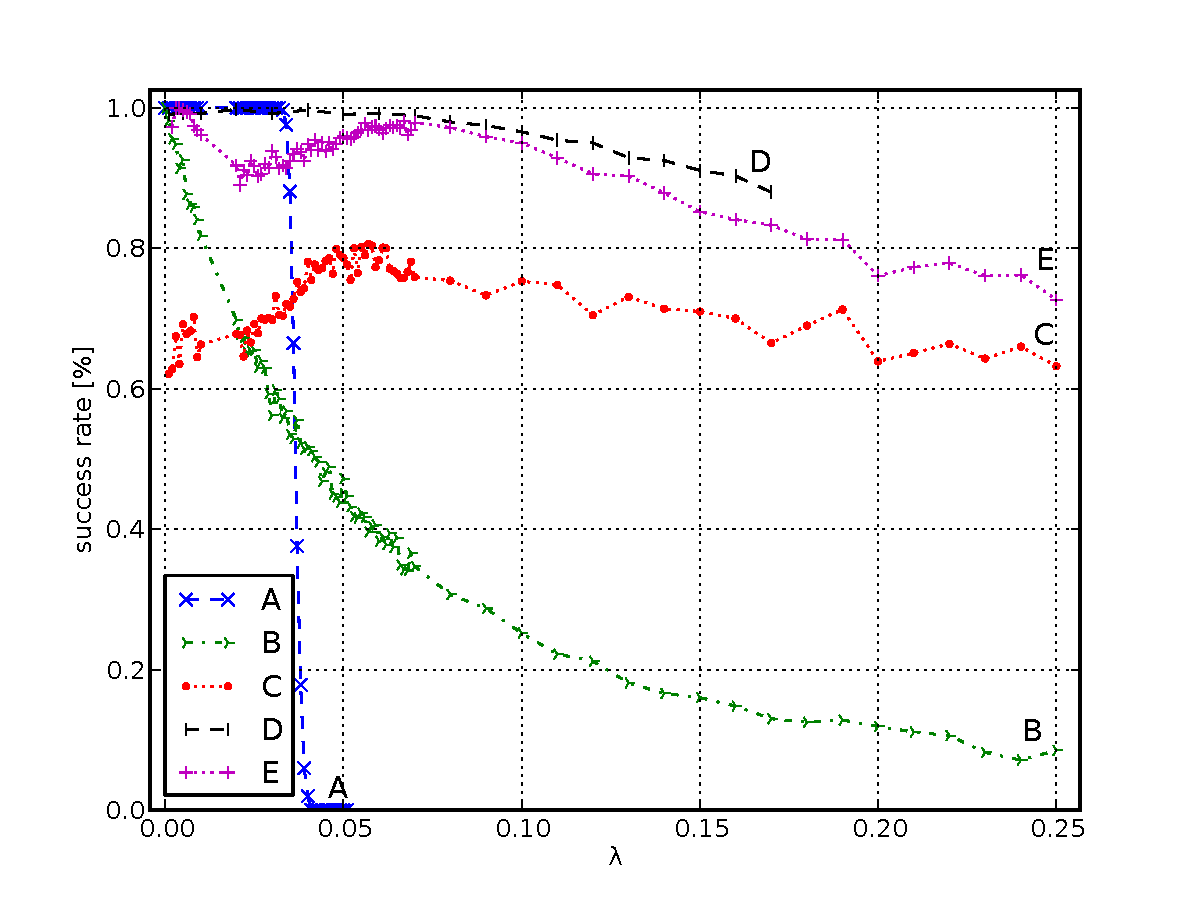
\includegraphics[width=\textwidth]{alg_1.pdf}}}
{\scalebox{0.43}{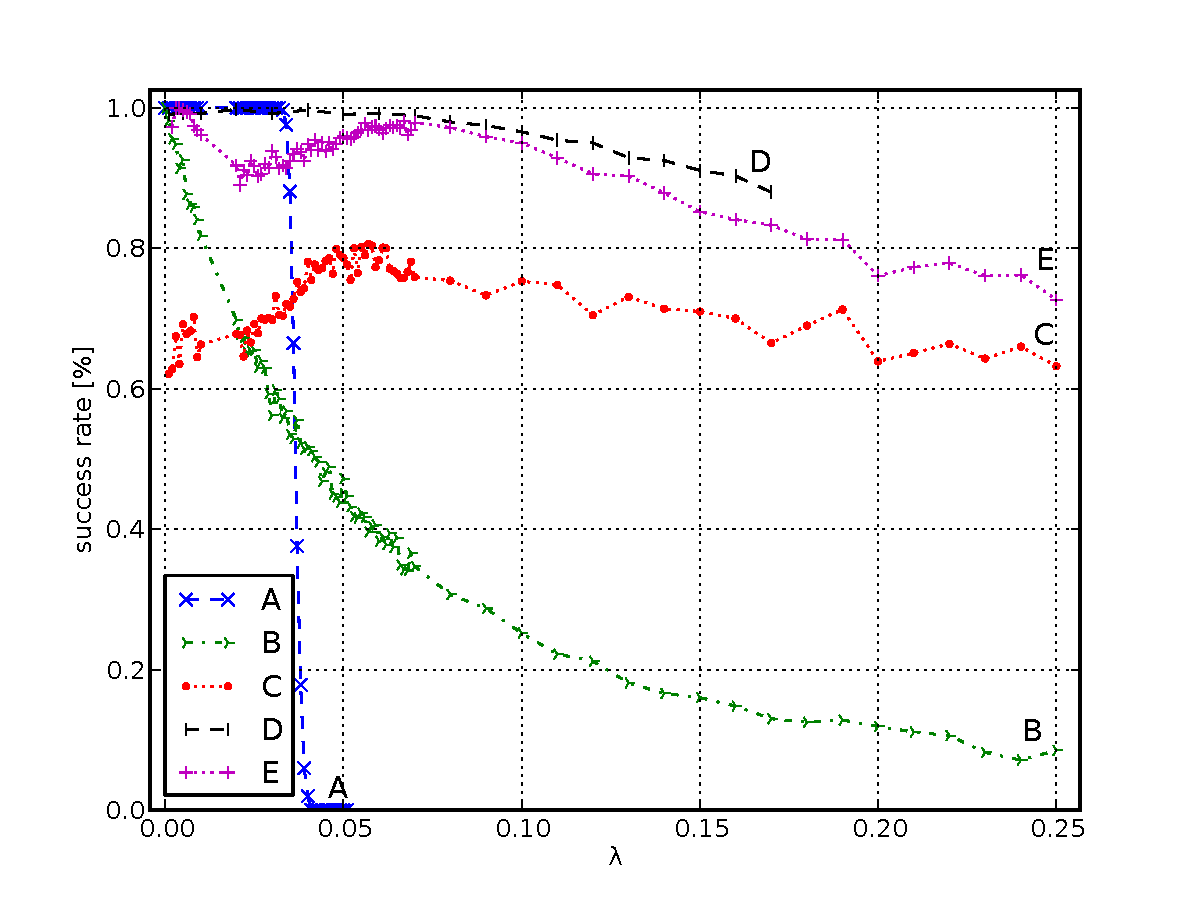
\includegraphics[trim=40 0 0 0]{alg_1.pdf}}}
% \end{center}
\caption{Algorithm evaluation in a simulation, $T=10~ms$. Number of a simulation rounds for one parameter setting is 1000.
 A, B, C correspond to the Algorithm I, II and III respectively.
 D, E correspond to the Algorithm IV with optimized $C(\lambda T)$ by an exhaustive search in D case, 
 in E case $C(\lambda T)$ is approximated by a polynomial.}
\label{fig:alg_eval}
\end{figure}
% \end{figure*}
% \end{wrapfigure}
    
\begin{figure}[H]
{\scalebox{0.43}{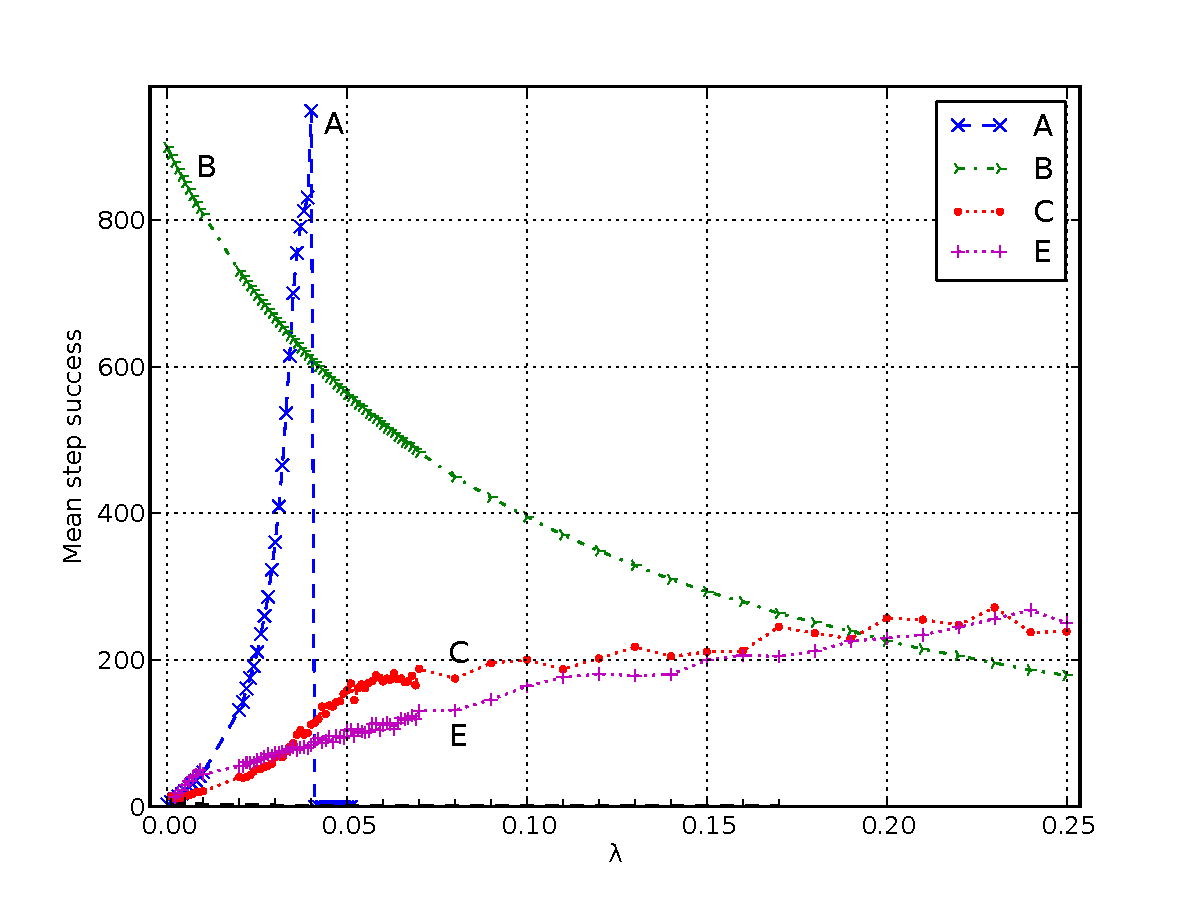
\includegraphics[trim=40 0 0 0]{alg_steps.pdf}}}
\caption{Steps of the algorithms needed to success on average w.r.t. $\lambda$. Algorithms denoted in a same way as in figure \ref{fig:alg_eval}.}
\label{fig:alg_steps}
\end{figure}
Figure \ref{fig:alg_eval} shows algorithms success rate w.r.t. $\lambda$. 
Figure \ref{fig:alg_steps} depicts number of steps needed 
to succeed on average. From figures it is visible Alg. I is more suitable for networks with low 
workload since has $100\%$ success rate for $\lambda \in [0, 0.035]$. Outside this interval 
Alg. I is not working and another solution has to be applied. The problem is new connections are
created faster than algorithm progresses.

Alg. II is set to have fixed $\Delta=900$, in order to maximize the success rate. The disadvantage of this
algorithm is that it waits on a particular destination port and if it is taken by another connection
the algorithm fails. 

Alg. IV has high success rate for 
noisy networks but is very sensitive on a $\lambda$ estimation what decreases practical usability 
if $\lambda$ changes quickly over time (non-homogeneous Poisson process). Closed form formula for $C(\lambda T)$ 
optimizing success rate and analytic derivation of the algorithm is still an open question. 

% \begin{itemize}
%  \item ToDo: fitting model to the real data from MU network
%  \item ToDo: evaluating algorithms on real data from MU network
% \end{itemize}

\section{Real data modeling}
Data collected in our university network by NetFlow probes were studied to test the correspondence to the Poisson process
w.r.t. newly created connections/allocations on NAT. NAT was simulated in our program using
NetFlow data to provide network traffic to the NAT. NetFlow data capture 1 hour of a network communication in two different
day hours (03 -- low peak, 13 -- high peak).

NAT state (newly opened connections in window $T=10, 50, 100~ms$)
was sampled multiple times in a row, Poisson and Negative Binomial distributions were fitted using Maximum Likelihood Estimation (MLE)
and goodness-of-fit test with Pearson $\chi^2$ test was performed with confidence level $\alpha=0.05$.

\begin{table*}[t]
  \centering
  % set, T, sample size, PoFit, NB Fit, sample mean, variance of sample mean, sample variance
  \begin{tabular}{| l | r | r | r | r | r | r | r |} % 
    \hline
    Set & T [ms] & Samples & Poisson r. [\%] & NBinom r. [\%] & $\overline{m}_{E[X]}$ &  $V[\overline{m}_{E[X]}]$  & $\overline{m}_{V[X]}$ \\ \hline \hline 
    \multirow{7}{*}{03} & \multirow{3}{*}{10}   & 100		& 2.977		& 1.667		& 0.5121        & 0.0228                    & 0.5321 \\ \cline{3-8}
      &      & 500      	& 5.637		& 0.920		& 0.4851        & 0.0086        & 0.5146 \\  \cline{3-8}
      &      & 1000     	& 10.294	& 1.579		& 0.4831        & 0.0068        & 0.5142 \\  \cline{2-8}
      & \multirow{3}{*}{50}     & 100     	& 6.543		& 2.276 	& 2.3707	& 0.2373 & 2.9969 \\ \cline{3-8}
      &      & 500     		& 25.180	& 7.194		& 2.3871        & 0.1053        & 3.1179 \\ \cline{3-8}
      &      & 1000    		& 52.174	& 23.188	& 2.3920        & 0.0696        & 3.1576 \\ \cline{2-8}
      & \multirow{2}{*}{100}  	& 100		& 8.914		& 3.911		& 4.7263        & 0.7031                    & 7.1496 \\ \cline{3-8}
      &      & 500     		& 57.746	& 9.859		& 4.7668	& 0.2876 	& 7.4667 					\\ \hline

    \multirow{2}{*}{13}  & \multirow{2}{*}{10}     & 100     & 5.191      & 1.824     & 2.6438       &  0.2695    & 3.0020 \\ \cline{3-8}
      &      & 500     & 20.368     & 2.829     & 2.6579       &  0.1025                    & 3.1495 \\ \hline
  \end{tabular}
  \caption{Results from NAT simulation on the real data captured from the university network. 
    The meaning of columns from the left is following: data set name, sampling time, number of samples collected,
    \% of cases rejecting hypothesis about Poisson distribution,  
    \% of cases rejecting hypothesis about Negative Binomial distribution,
    sample mean of sample mean of port samples,
    sample variance of sample mean of port samples,
    sample mean of variance of port samples.}
  \label{tab:1}
\end{table*}

Regarding data from set 13, during activity peak during the day, we conclude that if a number of samples 
is lower, e.g., 100, the process of a creating a new connection on NAT can 
be modeled as a time homogeneous Poisson process successfully (hypothesis rejected in $5.191\%$ of cases).
The time window the network was monitored in this case is $T \cdot 100 = 1000~ms$. 

If the number of samples is higher, e.g., 500, the time window of studied network traffic is longer and
in a real world scenario the probability that $\lambda$ is constant in time is low with the increasing length of the time
window. Due to this time homogeneous model is not strong enough, data is 
overdispersed what causes failure to fit Poisson distribution (hypothesis rejected in $20.368\%$ of cases). As suggested
in literature, Negative Binomial model fits better for overdispersed\footnote{The data overdispersion may be caused by dependent events on the network e.g., time-triggered updates downloading, etc...}
data (hypothesis rejected in $2.829\%$ of cases). 
The open question is how to make use of this model in NAT traversal.

For 100 samples the match with the model is satisfactory. Provided algorithm is able to run completely (including learning $\lambda$),
the proposed algorithms should work like in a simulation.

Regarding data from set 03, we can conclude that lower network workload causes more stable mean of sampled ports (MLE for Poisson distribution),
thus the Poisson distribution hypothesis is not rejected even in longer time intervals for an estimated $\lambda$. 


\section{Discussion}
For simplicity, we assumed that $\lambda$ is the same on both sides, the new challenges 
can arise if we allow different parameters on both sides that we haven't studied yet.

Another open question is to find a model that optimizes given task, i.e., establishing a direct
connection. We proposed a start step, to model the same process that occurs on the network, i.e.,
Poisson process, but this method requires setting a coefficient function $C(\lambda T)$ for which 
we don't have exact analytic explanation. This method is also very sensitive to parameter fluctuations
and thus not very practical for a real world networks. 

In our setting we assume $T=10~ms$ in order to minimize the speed of the evolution of a Poisson process.
Such short sending interval can cause some packets may get dropped on the path to the destination. But the 
important is whether they reach the local NAT in order to create a mapping in allocation table. As proposed 
in \citep{Wang:2006:RSN:1156422.1156550} it is possible to run the algorithm with $T=10~ms$ to create a mapping
and then re-run the algorithm with higher $T$, e.g., $T=100~ms$ in order to deliver packets to the destination
using created mapping and holes created in the previous round.

Success rate of the algorithm strongly relies on accurate measurements of the network 
properties the client resides in. They can be measured prior connection establishment 
from the point the client connects to the network, as is usually done in ICE and gather 
more information, build better network model and so on in this way.

%We ignored the cases where there are already some allocations on NAT from older connections
%on the port interval the NAT traversal algorithm is using.

Another problematic thing is if this algorithm is followed by a multiple host pairs on
the same network in the same time. They would artificially increase the network workload
causing it wouldn't follow Poisson distribution rendering our algorithms as not usable in
this case.

\section{Conclusion}
The aim of this work was to study problem of the NAT traversal from statistical point of view,
and to provide an algorithm with high success rate for networks with low workload that is easy to 
implement and requires little system resources. 
Several algorithms solving this problem were proposed but there are still some open questions remaining. 
Our goal was to find the algorithms that maximize success rate using only one source port strategies 
what can be used in further research, possibly in combination with previous multiple source port strategies.

We modeled the network workload as a Poisson process what we verified on real data by hypothesis testing.

We developed an application written in Python that simulates NAT and mentioned algorithms, computes
statistics for port distributions on NAT and simulates algorithms for different parameters. It
may be helpful for another researchers interested in this area so we published it in public domain
hosted on GitHub [URL:HERE].

To validate our results we implemented Android application using baby-step giant-step algorithm
to traverse symmetric carrier-grade NAT the mobile phone operator was using. The implementation
works according to expectations.

\appendix
\section{NAT classes}\label{sec:classes_appendix}
Definition of a Full cone NAT and Address restricted cone NAT as given in section \ref{sec:nat}.

\paragraph{Full cone NAT.} ~\\
Allocation table $\mathbb{AT} \subseteq \{ \mathbb{IP}_{in} \times \mathbb{PORT} \} \times \mathbb{PORT}$ holds associations between internal 
hosts socket and mapped external NAT port. 
% Rule is created once the connection from the internal host is initiated to an arbitrary external address.
Filtering rule is:
\begin{align*}
& PASS((\text{IP\textsubscript{ex}}, \text{PORT\textsubscript{ex}}, \text{IP\textsubscript{nat}}, \text{PORT\textsubscript{nat}} )) \Leftrightarrow \\
&  \exists \; \text{IP\textsubscript{in}} \in \mathbb{IP}_{in}, \; \text{PORT\textsubscript{in}} \in \mathbb{PORT}:\\
& ((\text{IP\textsubscript{in}}, \text{PORT\textsubscript{in}}), \text{PORT\textsubscript{nat}} ) \in \mathbb{AT}
\end{align*}
 
\paragraph{Address restricted cone NAT.} ~\\
Allocation table $\mathbb{AT} \subseteq \{\mathbb{IP}_{in} \times \mathbb{PORT} \times \mathbb{IP}_{ex}\} \times \mathbb{PORT}$ 
holds associations between internal hosts socket, external host IP address and mapped external NAT port. 
% Rule is created once the connection from the internal host is initiated to an arbitrary external address.
Filtering rule is:
\begin{align*}
& PASS((\text{IP\textsubscript{ex}}, \text{PORT\textsubscript{ex}}, \text{IP\textsubscript{nat}}, \text{PORT\textsubscript{nat}} )) \Leftrightarrow \\
&  \exists \; \text{IP\textsubscript{in}} \in \mathbb{IP}, \; \text{PORT\textsubscript{in}} \in \mathbb{PORT}:\\
& ((\text{IP\textsubscript{in}}, \text{PORT\textsubscript{in}}, \text{IP\textsubscript{ex}}), \text{PORT\textsubscript{nat}} ) \in \mathbb{AT}
\end{align*}

% -----
% Bibliography
%\bibliographystyle{unsrtnat}
\bibliographystyle{plainnat}
\bibliography{paper}

% \end{multicols}
\end{document}
